\chapter{Multispektralny system wizyjny}
\label{cha:multispectral}

%TODO Kilka zdań o zawratości rozdziału - szczególnie, że jest różnorodna.
%TODO 2 - podtrzymuję powyższe - 2-3 zdania co w rozdziale.


 
\section{Podczerwień}

Każde ciało, które ma temperaturę wyższą niż zero absolutne, emituje swoją powierzchnią promieniowanie, którego natężenie zwiększa się wraz z jej wzrostem.
%TODO 2 tak Pan to zamotał, że nie wiadomo do czego ,,jej,, się odnosi - temp. czy powierzchni
Dla każdej temperatury danego ciała istnieje charakterystyczna długość fali o~najwyższej wartości mocy promieniowania. 
Wraz z~jej wzrostem, ta częstotliwość przesuwa się w zakres fal widzialnych.
Można to zaobserwować, gdy stal osiąga wysoką temperaturę, co skutkuję emisją światła.
Zależność ta jest opisana prawem Plancka, które opisuję emisję promieniowania elektromagnetycznego przez ciało doskonale czarne.
Ciało doskonale czarne to wyidealizowane ciało fizyczne, które całkowicie pochłania padające na nie promieniowanie oraz emituje promieniowanie ściśle związane z jego temperaturą.
Wykres na rysunku \ref{fig:perfect_black} przedstawia tę zależność.

Mianem podczerwieni określa się promieniowanie elektromagnetyczne w zakresie fali o~długości od 0,75 $\mu m$ do 1000~$\mu m$. Wyróżnia się następujące pasma podczerwieni:
\begin{itemize}
\item Bliska podczerwień (NIR ang. \textit{near infrared}) w~zakresie 0,75 $\mu m$ do 1,4 $\mu m$.
\item Podczerwień fal krótkich (SWIR ang. \textit{short-wawelength infrared}) w~zakresie 1,4$\mu m$ do 3$\mu m$.
\item Podczerwień fal średnich (SWIR ang. \textit{mid-wavelength infrared}) w~zakresie 3$\mu m$ do 8$\mu m$.
\item Podczerwień fal długich (LWIR ang. \textit{long-wavelength infrared}) w~zakresie 8$\mu m$ do 15$\mu m$.
\item Daleka podczerwień (FIR ang. \textit{long-wavelength infrared}) w~zakresie 15$\mu m$ do 1000$\mu m$.
\end{itemize}

Bliska podczerwień znajduje się tuż za zakresem światła widzialnego ludzkim wzrokiem i~jest możliwa do rejestracji przez typowe dla kamer sensory CCD czy CMOS (często z~zastosowaniem dodatkowych oświetlaczy IR). 
Wraz ze wzmacniaczem światła jest również stosowana w~noktowizji.

SWIR i~LWIR występują także pod nazwą termowizji. 
Promieniowanie podczerwone jest częściowo pochłaniane przez atmosferę ziemską. 
Na rysunku \ref{fig:atmosfera_int} przedstawiono tzw. transmisyjność atmosfery. 
W~aparaturze rejestrującej w~podczerwieni wykorzystuje się dwa zakresy, przy których transmisyjność jest największa: 3 -- 5 $\mu m$ oraz 8 -- 14 $\mu m$ \cite{niklaus2007mems}.


\begin{figure}
\centering
\includegraphics[width=0.8\linewidth]{images/Atmosfaerisk_spredning}
\caption[Wykres transmisyjności atmosfery dla promieniowania podczerwonego ]{Wykres transmisyjności atmosfery dla promieniowania podczerwonego \cite{wiki:infrared}.}
\label{fig:perfect_black}
\end{figure}

\begin{figure}
\centering
\includegraphics[width=0.4\linewidth]{images/perfect_black_emi}
\caption[Emisyjność ciała idealnie czarnego]{Emisyjność ciała idealnie czarnego.}
\label{fig:atmosfera_int}
\end{figure}


\section{Kamera termowizyjna}

\subsection{Sensor podczerwieni}

W kamerach do rejestracji obrazu w termowizji są wykorzystywane sensory FPA (ang. \textit{Focal Plane Array} -- płaskie zespoły ogniskujące). 
Najbardziej popularne typy to: InSb, InGaAs, HgCdTe (w postaci fotodiod; wymagają kriogenicznych warunków pracy) and QWIP (ang. \textit{Quantum well infrared photodetector}). 
Najnowsze technologie wykorzystują niskobudżetowe, niewymagające chłodzenia mikrobolometry.
%TODO 2 A co to są te mikrobolometry ? Te chemiczne symoble, też może Pan nazwać.

Firma FLIR wykorzystuje tlenek wanadu do budowy mikrobolometrów m.in. w kamerach Lepton. 
Tlenek wanadu cechuje się dużym temperaturowym współczynnikiem rezystancji (TWR) oraz małym szumem 1/f, co zapewnia doskonałą czułość oraz jednolitość. 
W~celu uzyskania obrazu, zespół soczewek skupia promieniowanie z~rejestrowanej sceny na macierz detektorów. 
W~każdym z~detektorów, w~odpowiedzi na padającą na niego wiązkę promieniowania, zmienia się temperatura zawartego w~nim tlenku wanadu. 
Zmiana temperatury wiąże się proporcjonalnie ze zmianą rezystancji. 
Rejestracja sceny polega na odczycie rezystancji każdego detektora poprzez przyłożenia napięcia i~odczyt przepływającego przez nie prądu \cite{flir:lepton}.

%TODO 2 A może znajdzie Pan jakiś rysunek/schemat dla ożywnienia

\subsection{Kamera termowizyjna FLIR Lepton}
\begin{figure}[h]
\centering
\includegraphics[width=0.6\textwidth]{images/Lepton}
\caption{Widok poglądowy na kamerę FLIR Lepton.}
\label{fig:lepton}
\end{figure}

Lepton jest miniaturową kamerą termowizyjną. 
W~pojedynczym układzie został zintegrowany kompletny system składający się soczewki, sensora podczerwieni fal długich (ang. LWIR -- \textit{Long Wave Infrared}) oraz elektroniki sterującej i~przetwarzającej sygnał.
Kamera cechuje się bardzo małymi wymiarami, co czyni ją idealnym rozwiązaniem do zastosowań mobilnych.
Układ ma możliwość domontowania dodatkowej przesłony, która jest wykorzystywana do automatycznej optymalizacji procesu ujednolicania obrazu (kalibracji sensora).
Układ jest prosty do integracji z dowolnym mikrokontrolerem dzięki zastosowaniu standardowych protokołów i interfejsów. 

Lepton po podłączeniu zasilania od razu uruchamia się w~domyślnym trybie pracy. 
Kamera jest konfigurowalna poprzez CCI (ang. \textit{Camera Control Interface} – interfejs kontroli kamery).
Zapewnia on dostęp do rejestrów zawierających konfigurację \cite{lepton}. 

Parametry kamery:
\begin{itemize}
\item Wymiary: 11,8 x 12,7 x 7,2 mm, 
\item Sensor: niechłodzony mikrobolometr VOx (tlenek wanadu),
\item Rejestrowany zakres: fale długie podczerwieni, 8$\mu m$ do 14$\mu m$,
\item Wielkość piksela: 17 $\mu$m,
\item Rozdzielczość: 80x60 pikseli,
\item Liczba klatek na sekundę: 8,6,  
\item Zakres rejestrowanych temperatur: -10  $^\circ$  C 140  $^\circ$  C (tryb wysokiego wzmocnienia),
\item Korekta niejednorodności matrycy: automatyczna na bazie przepływu optycznego, 
\item Kąt widzenia horyzontalny / diagonalny: 51 $^\circ$  66 $^\circ$,
\item Głębia ostrości: od 10 cm do nieskończoności,
\item Format wyjściowy: do wyboru: 14-bit, 8-bit (z AGC (ang. \textit{automatic gain control} -- automatyczna kontrola wzmocnienia)) 24-bit RGB (z ACG i koloryzacją),
\item Interfejs wideo: VoSPI (Video over Serial Peripherial Interface),
\item Interfejs sterujący: CCI (zbliżony do I2C).
\end{itemize}


\begin{figure}
\centering
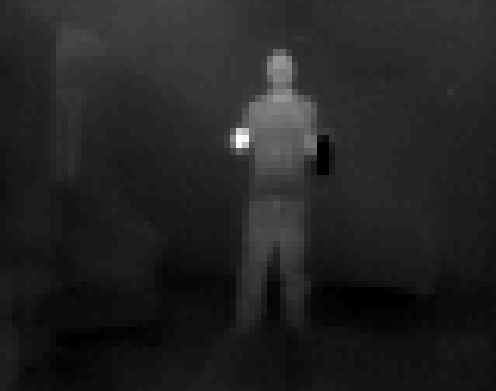
\includegraphics[width=0.5\linewidth]{images/leptonTermalImage.png}
\caption[Obraz człowieka w~termowizji wykonany kamerą Lepton.]{Obraz człowieka w termowizji wykonany kamerą Lepton. W~prawej ręce widać gorący obiekt (kubek herbaty), w~lewej zimny (butelka wody z lodówki).}
\label{fig:leptonTermalImage}
\end{figure}
%TODO 2 OK, ale tradycyjnie - powołanie w tekśie na obraz.



\section{Rejestracja obrazu multispektralnego}

Widmo elektromagnetyczne docierające do kamery składa się fal o~różnych długościach. 
Sensory w~kamerach rejestrują obraz tylko w~pewnym zakresie tego widma, więc aby uzyskać obraz w~wymaganym paśmie należy odfiltrować niepożądane elementy widma, np. kolorowy obraz z kamery wizyjnej jest otrzymywany poprzez zastosowanie trzech filtrów: czerwonego, zielonego i niebieskiego. 
Ponieważ wszystkie trzy kolory mogą być zarejestrowane przez pojedynczą matrycę, filtry są nałożone bezpośrednio na sensor, a~wartość koloru w danym punkcie jest interpolowana z~sąsiadujących ze sobą pikseli (tzw. matryca Bayera). 
W~przypadku, gdy nie jest możliwe zastosowanie jednego sensora do wszystkich pożądanych zakresów, należy rozdzielić wiązkę pomiędzy różne aparaty, albo wykorzystać równoległy układ kamer. %TODO 2 aparaty źle brzmi. Druga sprawa to są takie kamery 3x CMOS, gdzie wiązka jest rozdzialana na trzy czujniki (nie ma tej interpolacji)

W przypadku jednoczesnej rejestracji obrazu wizyjnego i~termicznego większość rozwiązań wykorzystuje układ dwóch równoległych do siebie kamer -- przykład przedstawia rysunek \ref{dual_camera}. 
W tym przypadku została zastosowana kamera termowizyjna FLIR Tao 2 oraz kamera wizyjna Logitech Webcam c600. 

Zazwyczaj obrazy z kamer różnią się, co wynika z ich budowy, różnej rozdzielczości, kąta widzenia oraz zniekształceń soczewkowych.
Do poprawnego odwzorowania tej samej sceny w~obu widmach należy zastosować algorytm mający na celu dopasowanie obu obrazów.
Tworzony jest w~ten sposób nowy obraz, na którym wszystkie piksele łączą informacje o~kolorze i temperaturze.

Pierwszym z~etapów poprawnego dopasowania obrazów jest kalibracja systemu wizyjnego.
Wykonuje się ją z~wykorzystaniem specjalnych plansz, które pozwalają określić położenie pewnych punktów w~przestrzeni w~obu rejestrowanych zakresach promieniowania.
Punkty te pozwalają na obliczenie relacji między obrazami.
Plansze mogą być aktywne (posiadają własne źródło ciepła) albo pasywne (przesłaniają obce źródło ciepła).
W~równoległym układzie kamer występuje również zjawisko paralaksy, które powiększa się wraz ze wzrostem odległości obiektu od punktu kalibracji. %TODO 2 to zdanie jest takie na doczepkę. Może napisać co z tego wynika

W~pracy \cite{hwang2015multispectral} autorzy zastosowali zwierciadło półprzezroczyste wykonane z~wafla krzemowego pokrytego cynkiem do rozdzielenia obrazu wizyjnego od termicznego (rysunek \ref{multispectral}). 
Wykorzystując trójosiowy uchwyt, kamery zostały ustawione tak, by ich osie optyczne się pokrywały. 
Następnie obrazy z~obu kamer zostały zrektyfikowane, aby miały tą samą wirtualną ogniskową.

\begin{figure}[h]
\centering
\begin{subfigure}{0.45\textwidth}
\centering
\includegraphics[width=1\textwidth]{images/dual-camera}
\subcaption{\label{dual_camera}}
\end{subfigure}
\begin{subfigure}{0.45\textwidth}
\centering
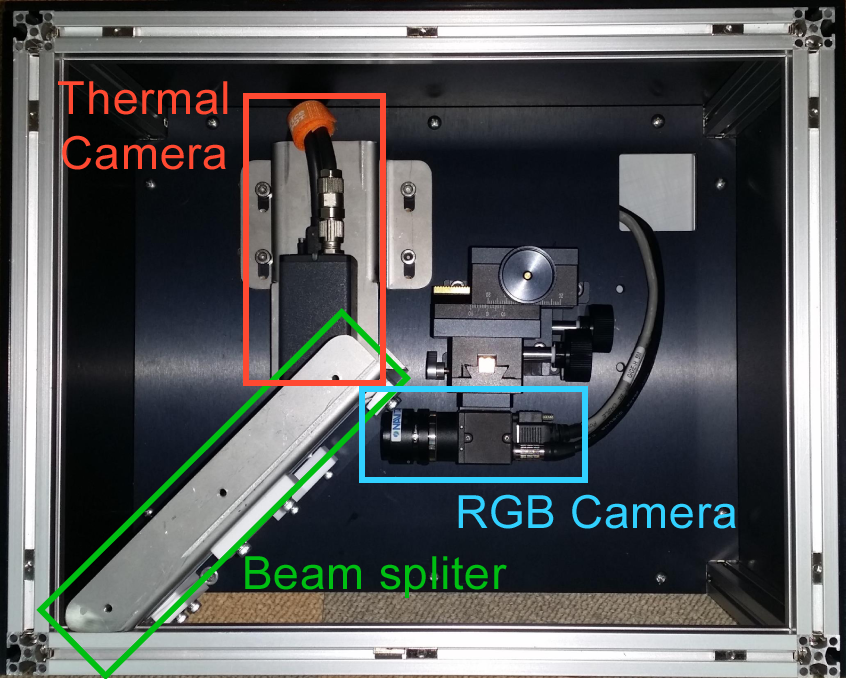
\includegraphics[width=1\textwidth]{images/multispectral}
\subcaption{\label{multispectral}}
\end{subfigure}
\caption{\label{fig:cameras_systems}Sposoby akwizycji obrazów: \protect\subref{dual_camera} dwie kamery równolegle \cite{lee2015robust}, \protect\subref{multispectral} z wykorzystaniem zwierciadła półprzezroczystego \cite{hwang2015multispectral}.}
\end{figure}


\subsection{Model geometryczny}

Do opisu matematycznego systemu wykorzystuje się model kamery otworkowej.
Dzięki niemu można opisać relację między trójwymiarową przestrzenią a~dwuwymiarowym obrazem za pomocą projekcji perspektywicznej. Nie stanowi on najdokładniejszego opisu matematycznego kamery, nie ma w nim uwzględnionych zakłóceń soczewkowych, jednakże zapewnia dobre rezultaty w~większości aplikacji.
Model składa się z~2 zestawów parametrów: zewnętrznych oraz wewnętrznych.
Parametry zewnętrzne definiują lokację kamery względem zewnętrznego układu współrzędnych.
Są reprezentowane przez wektor translacji \(T\) między układem związanym z~kamerą \( \left ( X_{c},Y_{c},Z_{c}\right ) \)
a~zewnętrznym \(\left ( X,Y,Z\right )\).
Drugim parametrem jest macierz rotacji \( R \) (między osiami tych dwóch układów).
Punkt \(P = \left [ X,Y,Z \right ]^T \) będący w~zewnętrznym układzie współrzędnym ma swój odpowiednik w~układzie wewnętrznym, który można określić zależnością:

\begin{equation}
P_{c} = RP+T
\end{equation}

Właściwości optyczne kamery można przedstawić w~postaci macierzy kamery:
\begin{equation}
K = \begin{bmatrix}
f_x & 0 & x_0 \\ 
0 & f_y & y_0\\ 
0 &0 & 1
\end{bmatrix}
\end{equation}
gdzie:
\begin{conditions}
f_{x}, f_{y} & ogniskowa kamery wyrażona w liczbie pikseli, \\
x_{0},y_{0} & współrzędne punktu głównego. 
\end{conditions}

Macierz $K$ określa związek między znormalizowanymi współrzędnymi w~układzie odniesienia kamery danych wzorem \(x_n = \frac{X_c}{Z_c}, y_n = \frac{Y_c}{Z_c}\)  a~odpowiadającym im współrzędnymi punktów na obrazie \(u,v\):

\begin{equation}
\begin{bmatrix}
u \\
v \\
1
\end{bmatrix} = K \begin{bmatrix}
x_n \\
y_n \\
1
\end{bmatrix}
\end{equation}

\subsection{Kalibracja}

Obrazy, które przedstawiają tę samą scenę, ale zostały wykonane dwoma różnymi kamerami w~innych położeniach różnią się. 
Na rysunku \ref{fig:oneSceaneTwoCameras} czarna szachownica jest uchwycona przez dwie kamery ustawione w~punktach $C_A$ (na wprost obiektu) oraz $C_B$ (po skosie i~lekko obrócona).

\begin{figure}
\centering
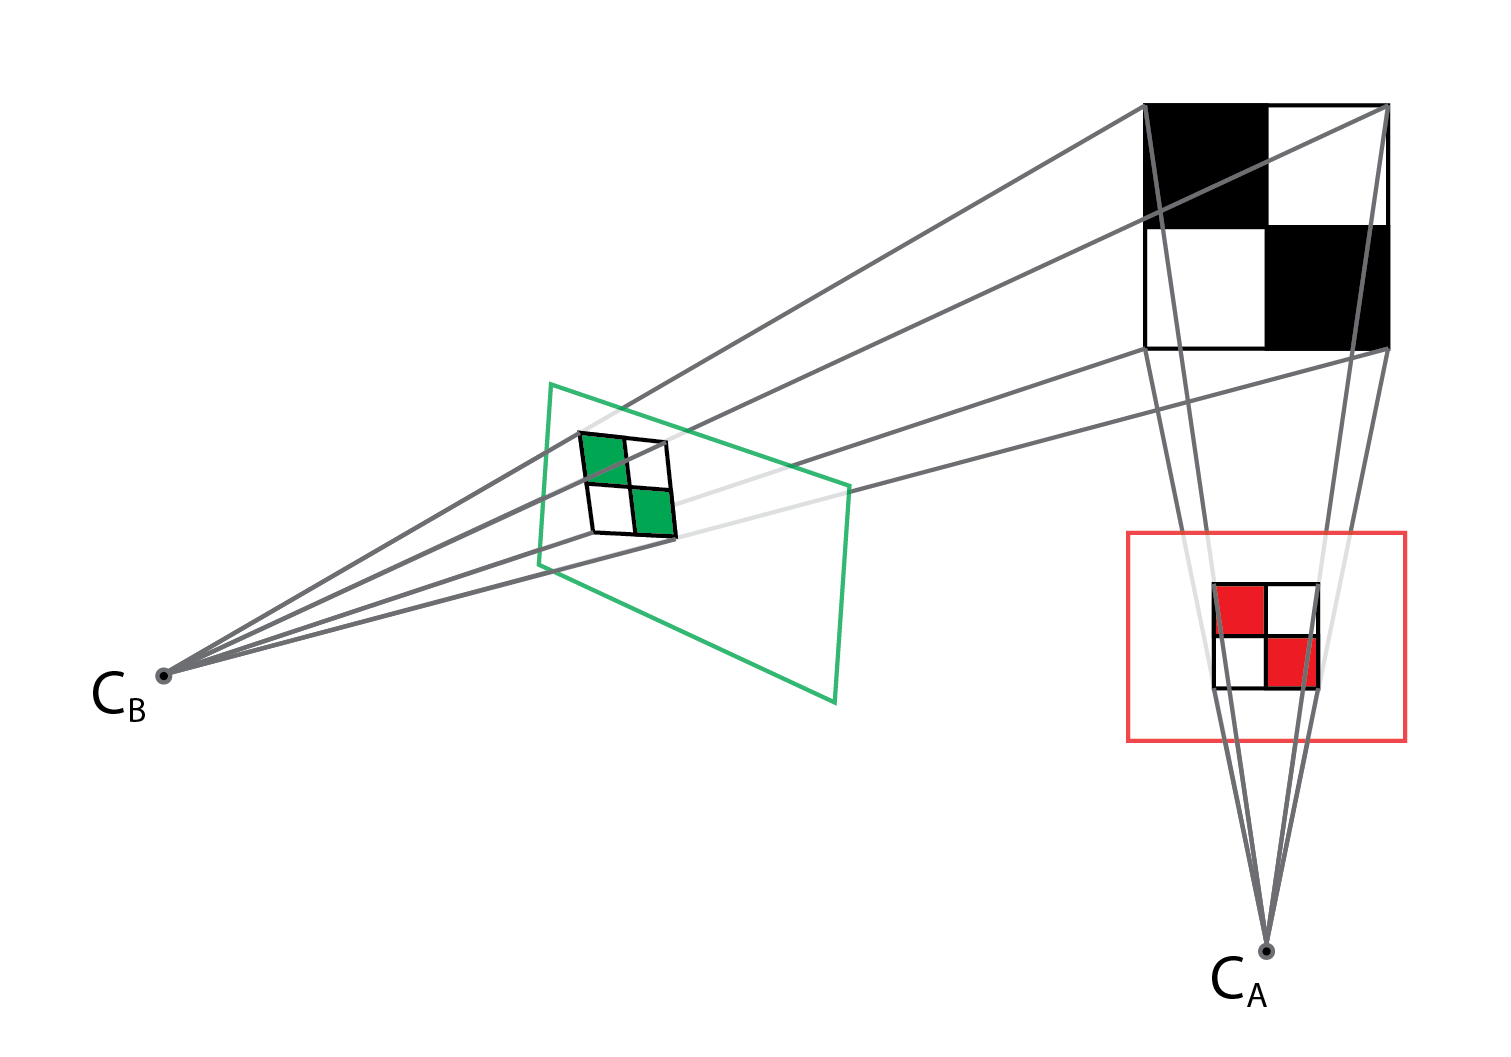
\includegraphics[width=0.6\linewidth]{images/oneSceaneTwoCameras}
\caption[Dwie kamery rejestrujące jeden obiekt. ]{Dwie kamery rejestrujące jeden obiekt.}
\label{fig:oneSceaneTwoCameras}
\end{figure}

Aby dopasować te dwa obrazy, tak by szachownice były ujęte tak samo (tj. w~tym samym miejscu na obrazie), należy na jednym z~nich przeprowadzić transformację projekcyjną. 
Jest to przekształcenie pomiędzy dwoma płaszczyznami, które wykorzystuje model geometryczny kamery. 
Wymaga to uprzedniego wyznaczenia macierzy transformacji $A$ na podstawie co najmniej 4 punktów kalibracyjnych.

\begin{figure}[h]
\centering
\begin{subfigure}{0.30\textwidth}
\centering
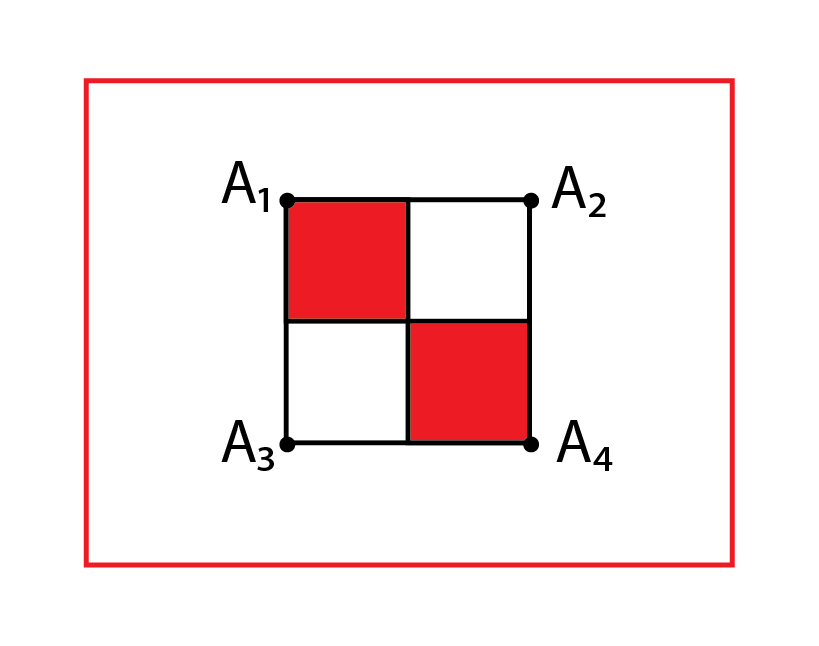
\includegraphics[width=1\textwidth]{images/camAimage}
\subcaption{\label{fig:camAimage}}
\end{subfigure}
\begin{subfigure}{0.30\textwidth}
\centering
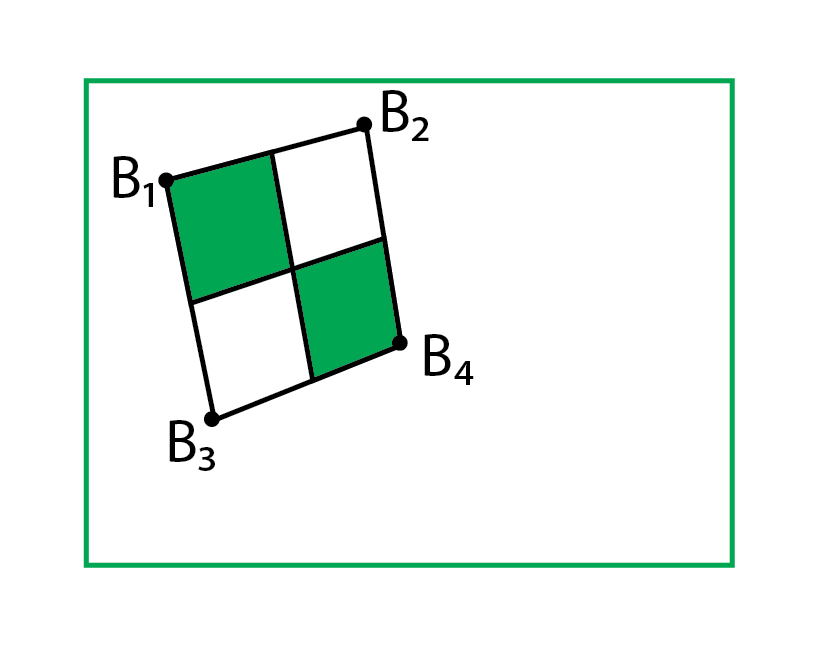
\includegraphics[width=1\textwidth]{images/camBimage}
\subcaption{\label{fig:camBimage}}
\end{subfigure}
\caption{\label{fig:camImages}Zarejestrowane obrazy: \protect\subref{fig:camAimage} przez kamerę $C_A$, \protect\subref{fig:camBimage} przez kamerę $C_B$. Punkty $A$ i $B$ są punktami kalibracyjnymi.}
\end{figure}

Na rysunkach \ref{fig:camAimage} i~\ref{fig:camBimage} punkty $A_1$ do $A_4$, będące czterema rogami zarejestrowanej szachownicy przez kamerę $C_A$, odpowiadają punktom $B_1$ do $B_4$, będącymi tymi samymi czterema rogami zarejestrowanymi kamerą $C_B$. Macierz transformacji $A$ można obliczyć rozwiązując równanie \eqref{transformMatrix}:
\begin{equation}
\label{transformMatrix}
A = \begin{bmatrix}
a & b & c\\ 
d & e & f\\ 
g & h & 1
\end{bmatrix}
\end{equation}

\begin{equation}
\begin{bmatrix}
u_1\\ 
u_2\\ 
u_3\\ 
u_4\\
...\\ 
u_n\\ 
v_1\\ 
v_2\\ 
v_3\\ 
v_4\\ 
...\\ 
v_n 

\end{bmatrix}
=
\begin{bmatrix}
x_1 & y_1 & 1 & 0 & 0 & 0 & -u_1x_1 & -u_1y_1\\ 
x_2 & y_2 & 1 & 0 & 0 & 0 & -u_2x_2 & -u_2y_2\\ 
x_3 & y_3 & 1 & 0 & 0 & 0 & -u_3x_3 & -u_3y_3\\ 
x_4 & y_4 & 1 & 0 & 0 & 0 & -u_4x_4 & -u_4y_4\\ 
...\\ 
x_n & x_n & 1 & 0 & 0 & 0 & -u_nx_n & -u_ny_n\\ 
0 & 0 & 0 & x_1 & y_1 & 1 & -v_1x_1 & -v_1y_1\\ 
0 & 0 & 0 & x_2 & y_2 & 1 & -v_2x_2 & -v_2y_2\\  
0 & 0 & 0 & x_3 & y_3 & 1 & -v_3x_3 & -v_3y_3\\ 
0 & 0 & 0 & x_4 & y_4 & 1 & -v_4x_4 & -v_4y_4\\ 
...\\ 
0 & 0 & 0 & x_n & y_n & 1 & -v_nx_n & -v_ny_n
\end{bmatrix}
\begin{bmatrix}
a \\
b\\
c\\
d \\
e\\
f\\
g\\
h
\end{bmatrix}
\end{equation}

\begin{conditions}
u_{n},v_{n} & współrzędne punktu kalibracji $n$, na obrazie bazowym\\
x_{n},y_{n} & współrzędne punktu kalibracji $n$, na obrazie dopasowywanym 
\end{conditions}

Transformację projekcyjną można zinterpretować jako rzutowanie płaszczyzny, co obrazuję rysunek \ref{fig:projection}. 
Wynikiem transformacji (a~zarazem rzutowania) jest obraz dopasowany do obrazu bazowego (\ref{fig:projectionImage})


\begin{figure}
\centering
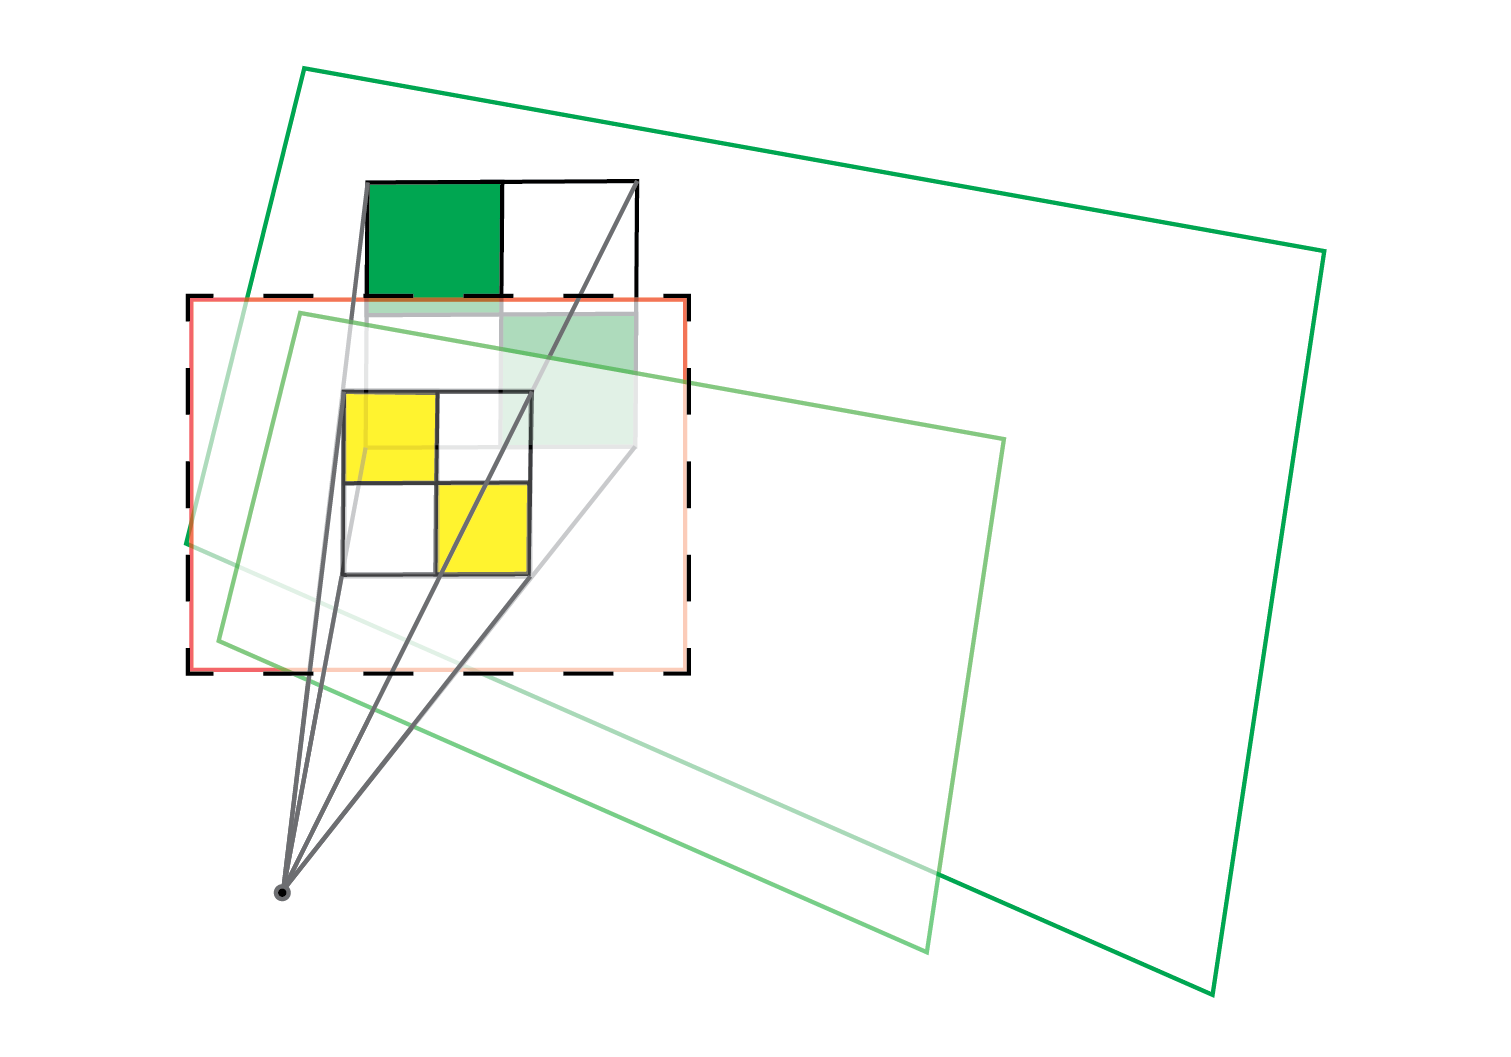
\includegraphics[width=0.6\linewidth]{images/projection}
\caption[Interpretacja transformacji projekcyjnej: rzutowanie płaszczyzny. ]{Interpretacja transformacji projekcyjnej: rzutowanie płaszczyzny.}
\label{fig:projection}
\end{figure}

\begin{figure}
\centering
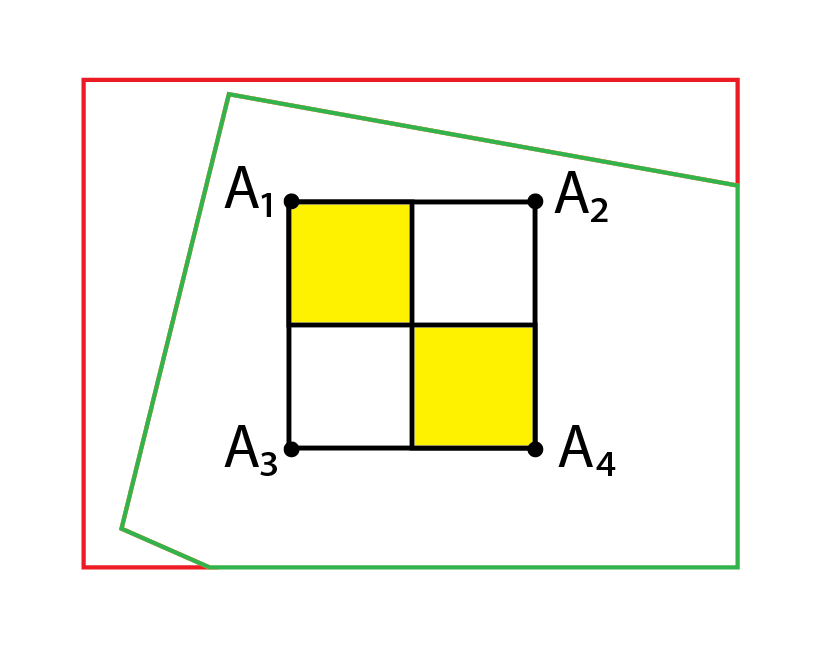
\includegraphics[width=0.30\linewidth]{images/projectionImage}
\caption[Wynik transformacji. ]{Wynik transformacji.}
\label{fig:projectionImage}
\end{figure}
